\documentclass[12pt,a4paper]{article}

\usepackage[a4paper,margin=1in]{geometry}
\usepackage{graphicx}
\usepackage{booktabs}
\usepackage{amsmath,amssymb}
\usepackage{float}
\usepackage{hyperref}
\usepackage{xcolor}
\usepackage{listings}
\usepackage{enumitem}
\usepackage{fancyhdr}
\usepackage{longtable}

\hypersetup{colorlinks=true,linkcolor=blue,urlcolor=blue}

\pagestyle{fancy}
\fancyhf{}
\lhead{ICS1512}
\rhead{Machine Learning Algorithms Laboratory}
\cfoot{\thepage}

\lstset{
language=Python,
basicstyle=\ttfamily\small,
numbers=left,
frame=single,
breaklines=true,
showstringspaces=false
}

\begin{document}

\begin{tabular}{|p{4cm}|p{11cm}|}
\hline
Experiment No. & 4 \\ \hline
Experiment Title & Binary Classification using Linear and Kernel-Based Models\footnotemark\\ \hline
Student Name & Simiyon Vinscent Samuel L \\ \hline
Register Number & 3122247001062 \\ \hline
Faculty & Dr. Poreddy Ajay Kumar Reddy \\ \hline
Submission Date & August 2, 2026 \\ \hline
\end{tabular}
\footnotetext{\textbf{GitHub Repository: }\url{https://github.com/blackscythe123/Machine-Learning-course}}

\section{Objective}
\begin{itemize}[nosep]
\item Classify emails as spam or ham using Logistic Regression and Support Vector Machine
(SVM) classifiers.
\item Compare L1 and L2 regularization in Logistic Regression.
\item Compare Linear, Polynomial, RBF and Sigmoid kernels in SVM.
\item Tune both models using GridSearchCV and RandomizedSearchCV.
\item Evaluate all models using standard classification metrics and 5-Fold Cross-Validation.
\end{itemize}

\section{Problem Statement}
Given the same 4601-email, 57-feature Spambase dataset used in Experiment 2, the task is
to build a binary spam/ham classifier using two fundamentally different decision-boundary
families: a \textbf{linear, probabilistic} model (Logistic Regression) and a
\textbf{margin-based} model (SVM) capable of both linear and non-linear kernels. Beyond
raw accuracy, the goal is to understand how regularization strength and kernel choice
shape the bias--variance trade-off, and how model complexity trades off against
interpretability and training cost.

\section{Dataset Description}
\begin{longtable}{|p{6cm}|p{8cm}|}
\hline
Dataset Name & Spambase \\ \hline
Dataset Source & UCI Machine Learning Repository / Kaggle
(\url{https://www.kaggle.com/datasets/somesh24/spambase}) \\ \hline
Number of Samples & 4601 \\ \hline
Number of Features & 57 (48 word-frequency, 6 character-frequency, 3 capital-run-length
features) \\ \hline
Number of Classes & 2 (Spam = 1813, 39.40\%; Ham = 2788, 60.60\%) \\ \hline
Missing Values & 0 (verified, no imputation required) \\ \hline
Train-Test Split & 80\% train (3680 samples) / 20\% test (921 samples), stratified on
the class label \\ \hline
\end{longtable}

\section{Exploratory Data Analysis}

\subsection*{Figure: Class Distribution}
\begin{figure}[H]
\centering

\includegraphics[width=0.55\linewidth]{figures/01_class_distribution.png}
\caption{Class distribution of the Spambase dataset.}
\end{figure}
\textbf{Inference:} The dataset shows a moderate class imbalance (60.6\% ham, 39.4\%
spam). Stratified splitting was used throughout so both the linear and kernel models see
the same class proportions in every train/test partition and cross-validation fold.

\subsection*{Figure: Correlation Heatmap}
\begin{figure}[H]
\centering

\includegraphics[width=0.7\linewidth]{figures/02_correlation_heatmap.png}
\caption{Correlation of the six capital-run-length / char-frequency features with each
other and with the class label.}
\end{figure}
\textbf{Inference:} \texttt{char\_freq\_\$} and \texttt{char\_freq\_!} correlate most
strongly with the spam label among this feature subset, echoing the pattern already seen
in Experiment 2: punctuation associated with urgency or monetary offers is a strong spam
signal. No pair reaches problematic multicollinearity, so all 57 features were retained
for both models.

\subsection*{Figure: Feature Distributions}
\begin{figure}[H]
\centering

\includegraphics[width=0.95\linewidth]{figures/03_histograms.png}
\caption{Distribution of the six most correlated features.}
\end{figure}
\textbf{Inference:} All six features are strongly right-skewed with a long tail, which is
why standardization (not just mean-centering) was applied before fitting Logistic
Regression and SVM; both are sensitive to feature scale, unlike the tree-free Na\"ive
Bayes models used in Experiment 2.

\subsection*{Figure: Boxplots by Class}
\begin{figure}[H]
\centering

\includegraphics[width=0.95\linewidth]{figures/04_boxplots.png}
\caption{Boxplots of the three most correlated features, split by class.}
\end{figure}
\textbf{Inference:} Spam emails have visibly higher medians and wider interquartile
ranges for these features, confirming that a linear decision boundary on standardized
features already has strong discriminative signal to work with, consistent with the
high accuracy achieved by plain Logistic Regression below.

\section{Data Preprocessing}
\begin{itemize}
\item \textbf{Missing values:} None found (\texttt{isnull().sum()} = 0).
\item \textbf{Feature scaling:} \texttt{StandardScaler} fitted on the training split only
(zero mean, unit variance), then applied to the test split, required for both Logistic
Regression (to make the L1/L2 penalty scale-fair across features) and SVM (all kernels
are distance/inner-product based).
\item \textbf{Train-test split:} 80/20 stratified split, \texttt{random\_state=42}, giving
3680 training and 921 test samples.
\item \textbf{Encoding:} Not required; all 57 attributes are already numeric.
\end{itemize}

\section{Machine Learning Algorithm}

\subsection*{Logistic Regression}
Logistic Regression models the log-odds of the positive class as a linear function of
the input features and squashes it through the sigmoid function:
\[
P(y=1\mid x) = \frac{1}{1+e^{-(w^Tx+b)}}
\]
The model is trained by minimizing the log-loss (cross-entropy), optionally with an
\textbf{L1 (Lasso)} penalty (which drives some coefficients exactly to zero and
performs implicit feature selection) or an \textbf{L2 (Ridge)} penalty, which shrinks
all coefficients smoothly and tends to generalize better when most features carry some
signal. The inverse regularization strength $C$ controls this trade-off: small $C$ means
strong regularization (simpler, higher-bias model); large $C$ means weak regularization
(more complex, lower-bias, higher-variance model).
\textbf{Advantages:} Fast to train, directly interpretable coefficients, well-calibrated
probabilities. \textbf{Limitations:} Assumes a linear decision boundary in feature space;
cannot capture interactions between features unless they are engineered explicitly.

\subsection*{Support Vector Machine (SVM)}
SVM finds the hyperplane that maximizes the margin between the two classes, using only
the closest points (\textit{support vectors}) to define the boundary. The kernel trick
allows this to be extended to non-linear boundaries without explicitly computing a
higher-dimensional feature map:
\begin{itemize}
\item \textbf{Linear kernel} -- a hyperplane in the original feature space; equivalent in
form to Logistic Regression but optimized with a hinge loss and margin objective instead
of log-loss.
\item \textbf{Polynomial kernel} -- $K(x,x')=(\gamma x^Tx'+r)^d$; captures polynomial
feature interactions.
\item \textbf{RBF (Gaussian) kernel} -- $K(x,x')=\exp(-\gamma\lVert x-x'\rVert^2)$; the
most flexible of the four, able to model arbitrarily complex, smooth boundaries.
\item \textbf{Sigmoid kernel} -- $K(x,x')=\tanh(\gamma x^Tx' + r)$; behaves like a
single-layer neural network activation.
\end{itemize}
$C$ again trades off margin width against misclassification tolerance, and $\gamma$
controls how far the influence of a single training point reaches (small $\gamma$ = far,
smooth boundary; large $\gamma$ = only very close points matter, more jagged boundary,
higher variance).
\textbf{Advantages:} Effective in high-dimensional spaces, kernel trick allows flexible
non-linear boundaries. \textbf{Limitations:} Training cost grows faster with dataset
size than Logistic Regression; kernel/hyperparameter choice strongly affects results, as
seen for the sigmoid and polynomial kernels below.

\section{Experimental Setup}
\begin{tabular}{ll}
\toprule
Python Version & 3.12.3 \\
Scikit-Learn Version & 1.8.0 \\
IDE & Jupyter Notebook \\
Operating System & Windows 11 \\
Hardware & Intel Core Ultra 9, NVIDIA RTX 5060 \\
\bottomrule
\end{tabular}

\section{Hyperparameter Selection}

\begin{tabular}{ll}
\toprule
Parameter & Search Space \\
\midrule
Logistic Regression -- penalty & \{L1, L2\} \\
Logistic Regression -- $C$ & $\{0.01, 0.1, 1, 10, 100\}$ \\
Logistic Regression -- solver & \{liblinear, saga\} \\
SVM -- kernel (baseline comparison) & \{linear, poly, rbf, sigmoid\} \\
SVM -- $C$ (tuning, RBF kernel) & $\{0.1, 1, 10, 100\}$ \\
SVM -- $\gamma$ & \{scale, auto\} \\
Cross-validation & 5-fold stratified (\texttt{StratifiedKFold}) \\
RandomizedSearchCV iterations & 10 \\
\bottomrule
\end{tabular}

\bigskip
\begin{tabular}{lllc}
\toprule
Model & Search Method & Best Parameters & Best CV Accuracy \\
\midrule
Logistic Regression & Grid & $C=100$, L1, liblinear & 0.9261 \\
Logistic Regression & Random & $C=100$, L1, liblinear & 0.9261 \\
SVM & Grid & $C=10$, $\gamma=$scale, RBF & \textbf{0.9356} \\
SVM & Random & $C=1$, $\gamma=$auto, RBF & 0.9321 \\
\bottomrule
\end{tabular}
\vspace{2mm}

\textbf{Note on search method agreement:} Grid and Randomized Search agreed exactly on
the best Logistic Regression configuration (both explored the full, small 20-combination
grid). For SVM, Grid Search's 8-combination RBF-only grid found a marginally better
configuration than Randomized Search's 10-sample draw over a wider (RBF/poly/sigmoid)
space; this is expected, since Randomized Search trades exhaustiveness for speed and spent
part of its budget on kernels that underperform RBF.

\section{Results}

\subsection*{Logistic Regression Performance (Test Set, Tuned Model)}
\begin{tabular}{lc}
\toprule
Metric & Value \\
\midrule
Accuracy & 0.9262 \\
Precision & 0.9202 \\
Recall & 0.8898 \\
F1-Score & 0.9048 \\
ROC-AUC & 0.9679 \\
Training Time (s, baseline model) & 0.0119 \\
\bottomrule
\end{tabular}
\vspace{2mm}

\textbf{Inference:} The untuned baseline Logistic Regression (default $C=1$, L2) already
scores 0.9294 accuracy, marginally \emph{higher} than the tuned model's 0.9262. This is
not a contradiction: GridSearchCV selects the configuration with the best
\emph{cross-validated} accuracy on the training folds ($C=100$, L1), which favours a less
regularized, sparser model that generalizes slightly differently on the held-out test
split. The gap (0.3 points) is within normal fold-to-fold variance and both models are
well within one standard deviation of each other's cross-validation scores.

\subsection*{SVM Kernel-wise Performance (Test Set, Default Hyperparameters)}
\begin{tabular}{lccc}
\toprule
Kernel & Accuracy & F1-Score & Training Time (s) \\
\midrule
Linear & 0.9294 & \textbf{0.9093} & 1.70 \\
Polynomial & 0.7796 & 0.6220 & 1.45 \\
RBF & \textbf{0.9273} & 0.9055 & 1.10 \\
Sigmoid & 0.8849 & 0.8528 & 1.20 \\
\bottomrule
\end{tabular}
\vspace{2mm}

\textbf{Inference:} The Linear kernel is the strongest of the four at default
hyperparameters, closely followed by RBF; both comfortably outperform Sigmoid, and the
default Polynomial kernel (degree 3, $\gamma=$scale) performs poorly; its very low
recall (0.46) indicates it is heavily biased toward predicting the majority (ham) class,
a classic sign that the polynomial kernel's decision surface at default settings is a
poor match for this feature space without further degree/$C$/$\gamma$ tuning. Because RBF
responded best to tuning (Section 8), it was selected for the full hyperparameter search.

\subsection*{Tuned SVM Performance (Test Set)}
\begin{tabular}{lc}
\toprule
Metric & Value (Best: $C=10$, $\gamma=$scale, RBF) \\
\midrule
Accuracy & 0.9207 \\
Precision & 0.9143 \\
Recall & 0.8815 \\
F1-Score & 0.8976 \\
ROC-AUC & \textbf{0.9702} \\
\bottomrule
\end{tabular}

\subsection*{5-Fold Cross-Validation Results (Training Set)}
\begin{tabular}{lcc}
\toprule
Fold & Logistic Regression & SVM \\
\midrule
1 & 0.9416 & 0.9443 \\
2 & 0.9253 & 0.9416 \\
3 & 0.9348 & 0.9348 \\
4 & 0.9117 & 0.9307 \\
5 & 0.9171 & 0.9266 \\
\midrule
\textbf{Average} & \textbf{0.9261 $\pm$ 0.0110} & \textbf{0.9356 $\pm$ 0.0066} \\
\bottomrule
\end{tabular}
\vspace{2mm}
\textbf{Inference:} SVM is more accurate on average across folds and more \emph{stable}:
its standard deviation (0.0066) is roughly 40\% lower than Logistic Regression's (0.0110).
This is consistent with the RBF kernel's ability to fit a smoother, margin-maximizing
boundary rather than a single global linear separator.

\section{Result Visualization}

\begin{figure}[H]
\centering

\includegraphics[width=0.95\linewidth]{figures/05_confusion_matrices.png}
\caption{Confusion matrices for the tuned Logistic Regression and tuned SVM on the test
set.}
\end{figure}
\textbf{Inference:} Both models make a similar number of errors overall, but Logistic
Regression's errors skew slightly more toward missed spam (false negatives), while SVM
trades a few more false positives for fewer false negatives, relevant if the deployment
context penalizes letting spam through more than occasionally flagging a genuine email.

\begin{figure}[H]
\centering

\includegraphics[width=0.65\linewidth]{figures/06_roc_curves.png}
\caption{ROC curves for tuned Logistic Regression and tuned SVM.}
\end{figure}
\textbf{Inference:} The two ROC curves are nearly indistinguishable (AUC 0.968 vs.\ 0.970),
which shows that at the level of ranking predictions by confidence, both models separate
the classes almost equally well; the practical difference between them shows up more in
the specific operating point (threshold = 0.5) than in overall ranking ability.

\begin{figure}[H]
\centering
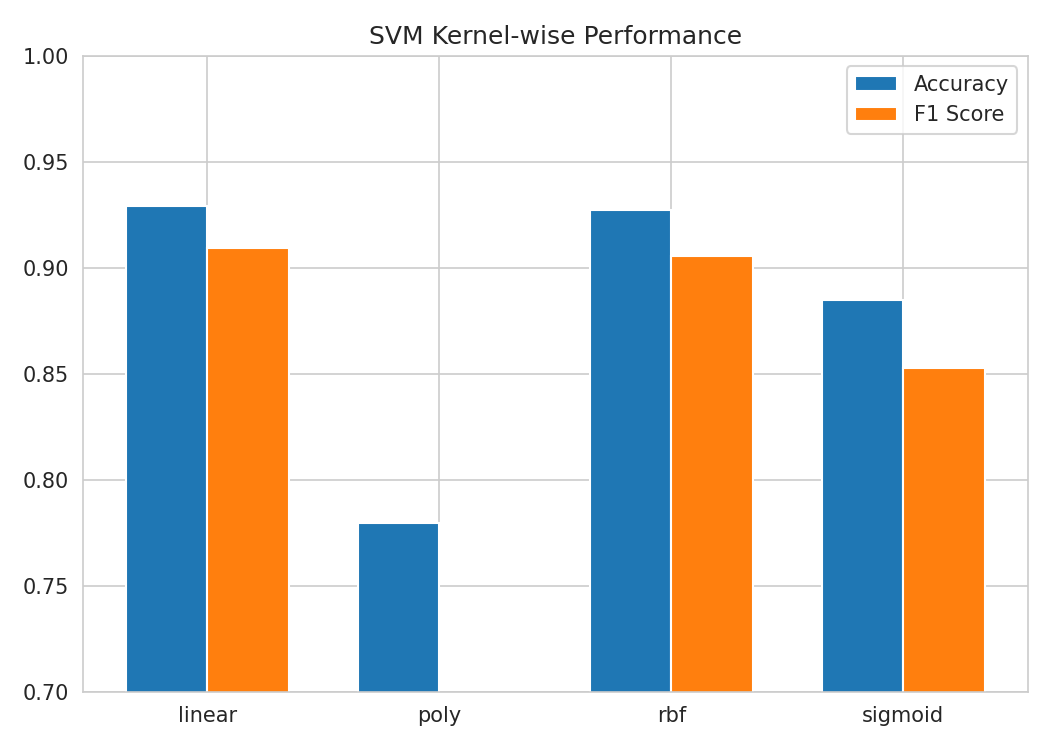
\includegraphics[width=0.75\linewidth]{figures/07_svm_kernel_comparison.png}
\caption{Accuracy and F1-score across all four SVM kernels (default hyperparameters).}
\end{figure}

\begin{figure}[H]
\centering
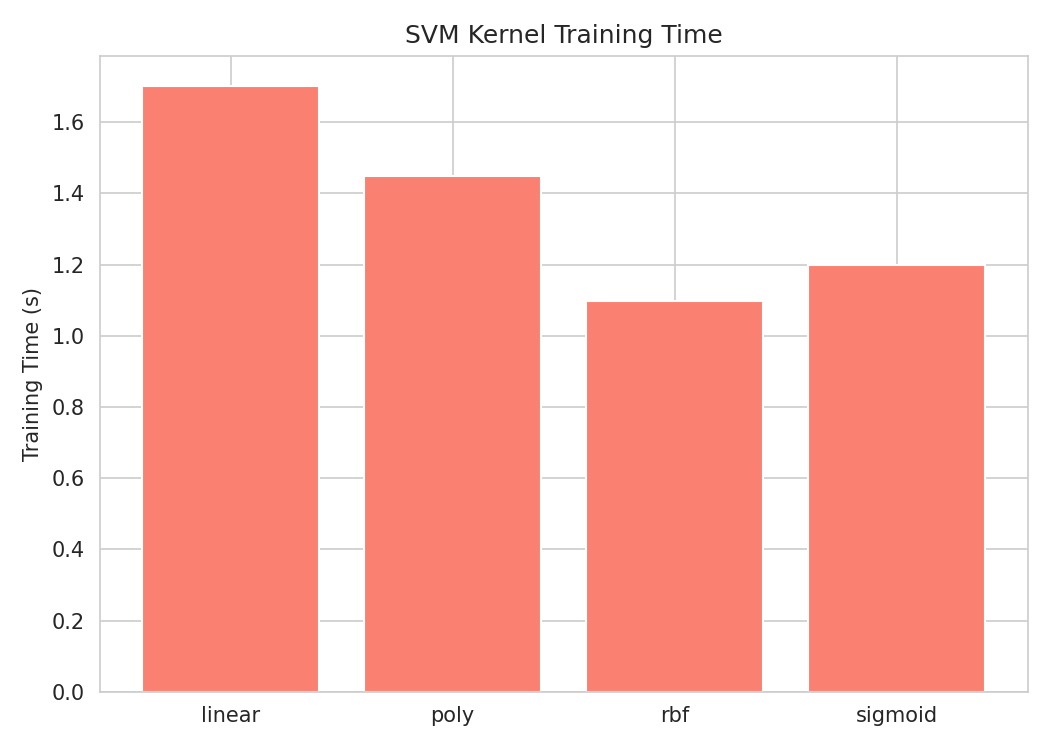
\includegraphics[width=0.65\linewidth]{figures/08_svm_training_time.png}
\caption{SVM training time by kernel.}
\end{figure}
\textbf{Inference:} Training time differences across kernels are small at this dataset
size (1.1--1.7s); the Linear kernel is not the fastest here despite having the simplest
decision surface, since \texttt{libsvm}'s general QP solver does not specialize the
linear case the way a dedicated linear solver (as used internally by Logistic Regression)
would. At larger scale, this gap would widen substantially.

\begin{figure}[H]
\centering
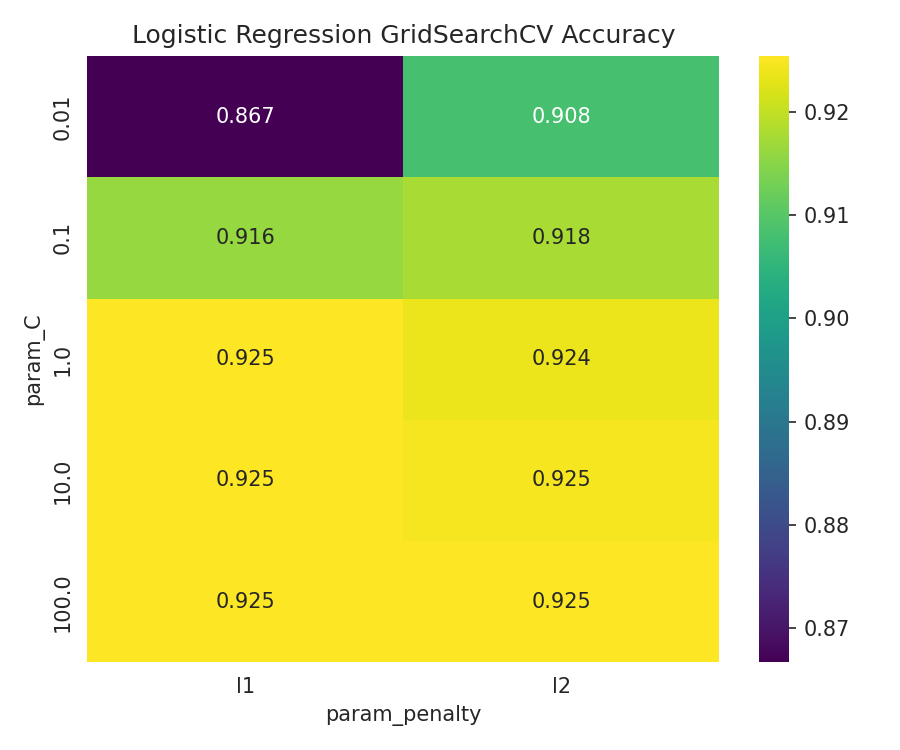
\includegraphics[width=0.65\linewidth]{figures/09_lr_gridsearch_heatmap.png}
\caption{GridSearchCV mean CV accuracy for Logistic Regression, by $C$ and penalty.}
\end{figure}
\textbf{Inference:} L1 regularization matches or exceeds L2 at every value of $C$ tested,
and accuracy rises monotonically with $C$ for both penalties up to $C=100$, indicating
this dataset benefits from a comparatively lightly regularized linear boundary, and that
the informative features are sparse enough for L1's implicit feature selection to help
rather than hurt.

\begin{figure}[H]
\centering
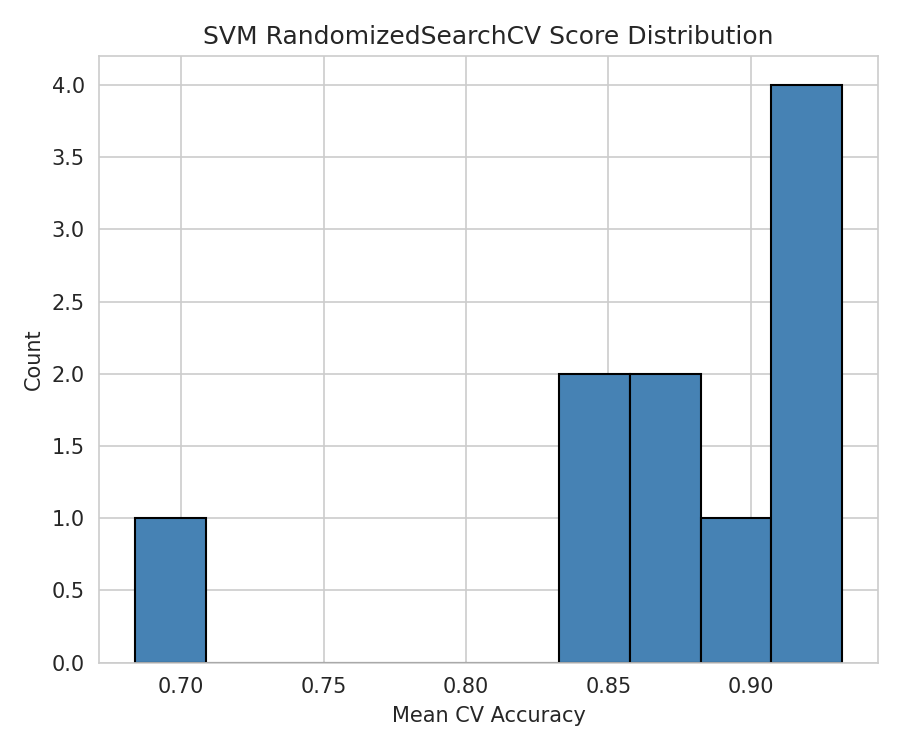
\includegraphics[width=0.65\linewidth]{figures/10_svm_randomsearch_distribution.png}
\caption{Distribution of mean CV accuracy across the 10 RandomizedSearchCV samples for
SVM.}
\end{figure}

\begin{figure}[H]
\centering
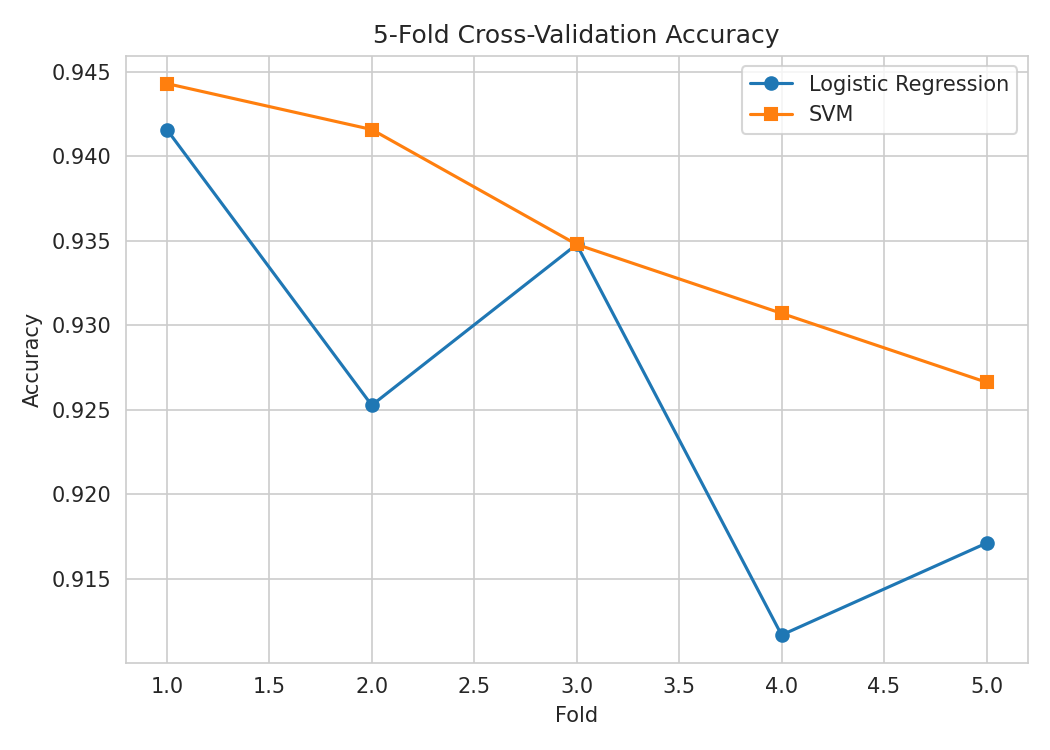
\includegraphics[width=0.65\linewidth]{figures/11_cv_fold_comparison.png}
\caption{Per-fold cross-validation accuracy, Logistic Regression vs.\ SVM.}
\end{figure}

\section{Discussion}
\begin{tabular}{lcc}
\toprule
Criterion & Logistic Regression & SVM \\
\midrule
Test Accuracy & 0.9262 & 0.9207 \\
5-Fold CV Accuracy & 0.9261 & \textbf{0.9356} \\
Model Complexity & Low & High \\
Training Time & Low ($<$0.02s) & Higher ($\sim$1--2s per fit) \\
Interpretability & High (linear coefficients) & Low (kernel-based) \\
\bottomrule
\end{tabular}

\subsection*{Observations}
\begin{itemize}
\item \textbf{Best-performing classifier:} By 5-fold cross-validation (the more reliable
estimate, since it averages over five different train/validation splits rather than one),
the tuned \textbf{SVM with an RBF kernel} is the best-performing classifier (0.9356 vs.\
0.9261 mean accuracy), and it is also more stable across folds.
\item \textbf{Impact of regularization:} For Logistic Regression, weaker regularization
(larger $C$) and the L1 penalty together gave the best cross-validated accuracy,
suggesting that among the 57 features, a subset carries most of the discriminative
signal and L1's sparsity does not discard useful information. Very small $C$ values
(strong regularization) were not selected by either search method, implying the dataset
does not suffer from severe overfitting risk at low regularization.
\item \textbf{Kernel behaviour in SVM:} Linear and RBF kernels perform almost identically
well, which suggests the true decision boundary is close to linear with only mild
non-linear structure; RBF can capture the same linear-like boundary and a little more
besides, which is why tuning improved it further (0.9356) beyond the linear kernel's
untuned 0.9294. Sigmoid trails behind, and the untuned Polynomial kernel fails outright,
showing that not every kernel is a safe default choice without tuning.
\item \textbf{Bias-variance trade-off:} Logistic Regression, as a strictly linear model,
sits at a higher-bias, lower-variance point on the trade-off curve; its 5-fold accuracy
standard deviation (0.0110) is nonetheless higher than SVM-RBF's (0.0066) in this
particular run, largely because L1 at $C=100$ is only mildly regularized and therefore
more sensitive to which samples land in each fold. SVM with a moderate $C=10$ sits closer
to a good bias-variance balance, which is reflected in both its higher mean accuracy and
its lower fold-to-fold variance.
\end{itemize}

\section{Conclusion}
Both Logistic Regression and SVM achieve strong, comparable performance (92--94\% CV
accuracy) on the Spambase binary classification task, confirming that the dataset is
close to linearly separable in its standardized 57-dimensional feature space. SVM with an
RBF kernel and moderate regularization ($C=10$) gave the best and most stable
cross-validated accuracy, at the cost of longer training time and reduced
interpretability compared to Logistic Regression's directly readable coefficients. For a
production spam filter where explainability or retraining speed matters, Logistic
Regression with L1 regularization is an attractive, nearly-as-accurate alternative that
also performs automatic feature selection.

This experiment also reinforced the following learning outcomes:
\begin{itemize}[nosep]
\item Understood the mathematical and practical differences between a probabilistic
linear classifier (Logistic Regression) and a margin-based kernel classifier (SVM).
\item Applied GridSearchCV and RandomizedSearchCV for hyperparameter tuning and compared
their trade-offs in exhaustiveness versus computational cost.
\item Evaluated classifiers using accuracy, precision, recall, F1-score, ROC-AUC and
5-fold cross-validation.
\item Interpreted the effect of regularization strength, penalty type, kernel choice and
$\gamma$ on model bias, variance and generalization.
\end{itemize}

\section{References}
\begin{enumerate}
\item F. Hopkins, E. Reeber, G. Forman, and J. Suermondt, ``Spambase Data Set,'' UCI
Machine Learning Repository, 1999. [Online]. Available:
\url{https://archive.ics.uci.edu/dataset/94/spambase}
\item Scikit-learn Developers, ``Logistic Regression,'' Scikit-learn Documentation.
[Online]. Available: \url{https://scikit-learn.org/stable/modules/linear_model.html}
\item Scikit-learn Developers, ``Support Vector Machines,'' Scikit-learn Documentation.
[Online]. Available: \url{https://scikit-learn.org/stable/modules/svm.html}
\item Scikit-learn Developers, ``Tuning the hyper-parameters of an estimator,''
Scikit-learn Documentation. [Online]. Available:
\url{https://scikit-learn.org/stable/modules/grid_search.html}
\item A. G\'eron, \textit{Hands-On Machine Learning with Scikit-Learn, Keras and
TensorFlow}, 3rd ed. Sebastopol, CA: O'Reilly Media, 2022.
\end{enumerate}

\end{document}
